\subsection{Overview}
\label{sec:overview}

\VT{In the intro/background we use "Docker hosts" instead of "Docker clients".
Need to pick one and be consistent. I prefer ``Docker hosts''}
\NZ{I think it's not necessarily docker hosts. we can pull an image without using
	 docker engine}
\VT{Make drivers emphasized in the background}
%\NZ{arg1}
\begin{figure*}[t]
	\centering
		%\begin{minipage}{0.225\textwidth}
			\centering
			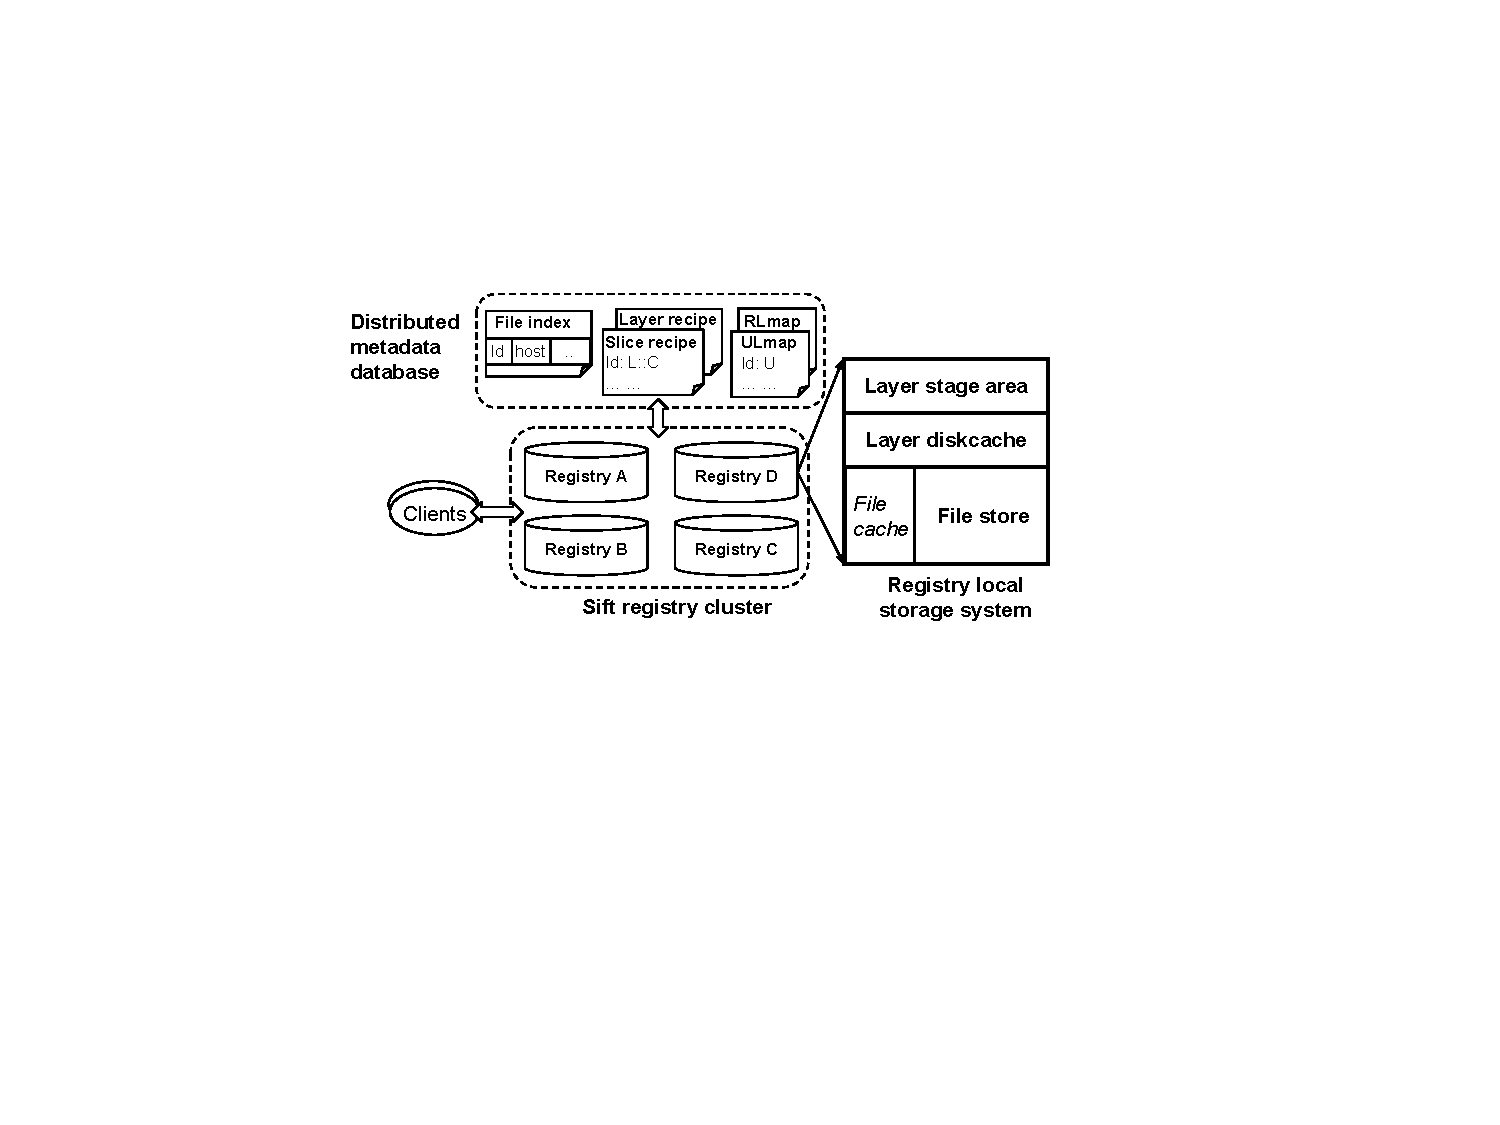
\includegraphics[width=0.9\textwidth]{graphs/sys-architecture.pdf}
%\vspace{-4pt}
			\caption{Architecture of \sysname.}
			%\label{fig:ref_count}
		%\end{minipage}
%	\begin{minipage}{0.225\textwidth}
%		\centering
%		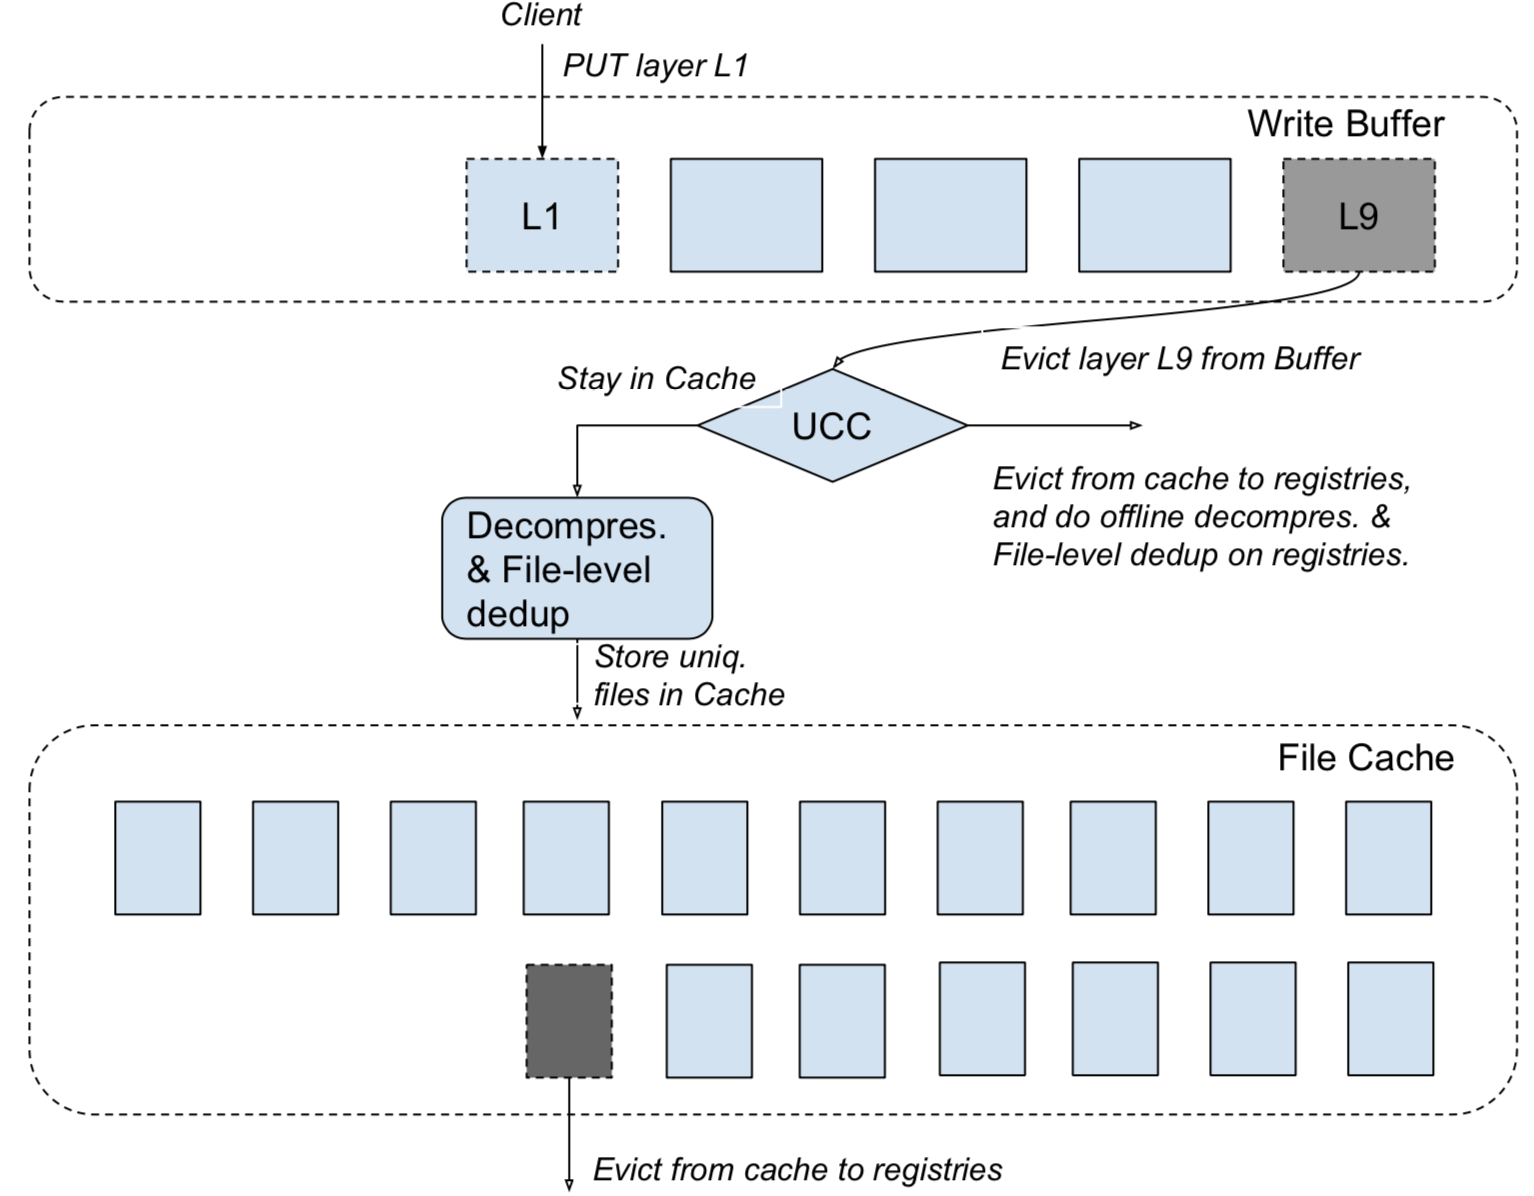
\includegraphics[width=1\textwidth]{graphs/slimmer-cache.png}
%		\caption{CDF of compress. and uncompress. layer size.}
%		\vspace{-3pt}
		\label{fig:sys-overview}
%\vspace{-4pt}
%	\end{minipage}
\end{figure*}


Figure~\ref{fig:sift} shows the architecture of \sysname.
%
\NZ{I think we can describe registry as a registry restful api. and indeed registry is a rest api}
\sysname consists of the two main components: %1)~\emph{frontend registries}, 
1)~a cluster of \emph{storage servers}
with registry RESTful API and 2)~a distributed
\emph{metadata database}. 
%\NZ{arg1}
%
When uploading or downloading layers, 
Docker clients communicate with the
registry RESTful API.
%
%As in the original registry, 
%\sysname registries are independent from each
%other.
%
Each server contains a registry RESTful API and a backend storage system.
%uses a \sysname driver that processes requests by
%communicatin with the metadata database and the backend storage servers.
%
Backend storage systems store
%manifests and
layers and perform deduplication, keeping the deduplication metadata in the
database.
%
%The metadata database keeps information necessary to deduplicate layers.
%
%To reduce deduplication overhead, \sysname tries to minimize the time it takes
%to restore a layer during a \texttt{pull} request.
%
\sysname uses three main techniques to reduce deduplication and restoring overhead:
1)~replica deduplication modes; 2)~parallel layer reconstruction; and
3)~predictive layer prefetching/preconstruction.




\paragraph{Replica deduplication modes.}
%
For higher fault tolerance and availability existing registry backends bluntly
replicate  each layer.
%
\sysname also performs replication, but some replicas it deduplicates while
keeping the remaining ones in the non-deduplicated state for faster downloads.

A \emph{basic deduplication mode} (B-mode) $n$ defines that \sysname should
keep $n$ layer replicas intact and deduplicate the remaining $R-n$ layer
replicas, where $R$ is the layer replication level.
%
\VT{Maybe call it B-mode n/R? R seems to be Sifts config parameter as well?}
%
At one extreme, B-mode $R$ means that no replica should be deduplicated and
hence, provides the best performance but no data reduction.
%
At the other end, B-mode $0$ deduplicates all layer replicas, i.e. it provides
the highest deduplication ratio but adds restoration overhead for every
\texttt{pull} request.
%
The remaining B-modes in between allow to trade off performance and data
reduction.
%
\VT{Do we replicate after deduplication? E.g., in B-mode 0 do we still have 
R replicas of all files for durability?}

\VT{Why keeping more than 1 non-deduped layers helps?}

For heavily skewed workloads, \sysname also provides a \emph{selective
deduplication mode} (S-mode).
%
The S-mode utilizes the skewness in layer popularity, observed
in~\cite{dockerworkload}, to decide, how many replicas should be deduplicated
for each layer individually.
%
As there are hot layers that receive the majority of \texttt{pull} requests,
S-mode sets the number of layer replicas inversely proportional to its
popularity.
%
This means that hot layers have less deduplicated replicas and
hence, can be served faster.
%
On the other hand, cold layers have more
deduplicated replicas to improve storage utilization.

Figure~\ref{fig:sift-original} shows an example for B-mode $1$ with $R=3$.
\sysname maintains a single layer replica (the \emph{primary layer replica}) on
server A for newly pushed layers.
%
The remaining two backup layer replicas are deduplicated, i.e. any duplicate
files are discard while unique files are kept.  The unique files are replicated
and saved on different servers B and C.
%
Any subsequent \texttt{pull} layer requests are sent to server A since it
stores a complete layer replica.
%
If server A crashes, server B or C is needed to rebuild the layer and serve the
\texttt{pull} request.
%
\VT{Why do we even have replicas of layers if we are the storage system,
so we control to have or not to have replicas?}
%
\VT{Wha tis original server in Figure~~\ref{fig:sift-original}? We never describe it
and how it works?}

To support the different deduplication modes, \sysname divides storage servers
into two groups (see Figure~\ref{fig:sift}): a \emph{primary cluster}
consisting of \emph{P-servers} and a \emph{deduplication cluster} consisting of
\emph{D-servers}.
%
P-servers are responsible for storing full layer replicas and manifest replicas
while D-servers deduplicate layer replicas at the file level, store the unique
files, and replicate them.
%
The split is necessary to ensure that layer replicas and its containing file
replicas are stored on different servers to maintain fault tolerance.


P-servers and D-servers form a two-tier storage hierarchy: In the default case,
the primary cluster serves all incoming \texttt{pull} requests.
%
If a request can't be served from the primary cluster, for example, due to a
node failure, it will forwarded to the deduplication cluster and the requested
layer will be restored.
%
\LR{Here we also need to talk about dealing with overloaded (not just crashed)
P-servers.}
%
\NZ{We use the superfetch cache on registry side instead of on backend storage
system to save some workload overhead to backend storage system.}





\paragraph{Parallel layer reconstruction.}
%
\sysname speeds up layer reconstruction through parallelism.
%
As shown in Figure~\ref{fig:sift}, each D-server's local storage is divided
into three parts: layer stage area, preconstruction cache, and file store.
%
The layer stage area temporarily stores newly added layer replicas.
%
After deduplicating a replica, the resulting unique files are stored in a
content addressable file store and replicated to the peer servers to provide
redundancy. Once all replicas have been stored, the layer replica is deleted
from the layer stage area and cached in the preconstruction cache.
%
The cache is also used to hold preconstructed
layers~(see~\S\ref{sec:cache-design}).

\sysname distributes the layer's unique files onto several servers
(see~\S\ref{sec:dedup-desgin}).
%
All files on a single server belonging to the same layer are called a
\emph{slice}.
%
A slice has a corresponding \emph{slice recipe}, which defines the files that
are part of this slice, and a \emph{layer recipe} defines the slices needed to
reconstruct the layer.
%
This information is stored in \sysname{}'s metadata database for reliability,
consistency, and fast accesses. 
%
This allows D-servers to rebuild layer slices in parallel and thereby, improve
reconstruction performance.
%
To avoid storing duplicate layers and keep track of already stored unique
files, \sysname maintains a layer and a file index. These are also kept in the
metadata database.




\paragraph{Predictive cache prefetching.}
%
To improve the layer access latency, \sysname employs a cache layer in both the
primary and the deduplication cluster.
%
Each P-server has an in-memory \emph{user-behavior based superfetch cache} to
reduce disk I/Os.
%
When a \texttt{pull} manifest request is received from a user, \sysname
predicts which layers in the image will actually need to be \texttt{pulled} and
\emph{prefetches} them in the cache.
%
To do that, \sysname maintains two maps: \emph{RLmap} and \emph{ULmap}.
%
RLmap stores the mapping between images and layers while ULmap keeps track of a
user's access history, i.e. which layers the user has pulled and how many
times~(see details in~\S\ref{sec:cache-design}).

Additionally, to avoid layer restoring overhead,
each D-server maintains an on-disk layer cache (called \emph{user-behavior based preconstruct cache}).
%
As with the superfetch cache algorithm,
when a \texttt{pull} manifest request is received,
\sysname predicts which layers in the image will be \texttt{pulled},
preconstructs the layers, and loads them in the preconstruct cache.
%
As shown in Figure~\ref{fig:intervals}, the time between a \texttt{GET} manifest request and its
subsequent \texttt{GET} layer request is more than 1\,s on average \todo{Give more specifics,
i.e. 50th percentile for different workloads}. As we will show in~\S\ref{sec:eval-dedup}, this is
sufficient to preconstruct the necessary layers and load them into the cache.
